When it comes to whitebox attacks, three approaches are evaluated: FGSM, CW and JSMA. Hyperparameters used in the FGSM and the CW attack are listed in Table \ref{table:fgsm-params} and Table \ref{table:cw-params}, respectively. In Table \ref{table:whitebox-fgsm-results} and \ref{table:whitebox-cw-results} results are presented for FGSM attack and CW attack, respectively. In Table \ref{table:whitebox-results} results of all three attacks are presented.

It is interesting to notice that the FGSM attack managed to change MAE for the model with id 2 from 9.5 to 47.79. In other words, the targeted model on average predicted that a person in the adversarial image is 38 years younger or older than a person in the original image! 

Several original samples and the corresponding adversarial samples crafted in this experiment are presented in Figure \ref{fig:fgsm-attack}. It can be observed that the attack adds a similar pattern to every image. However, when hyperparameter $eps$ is reduced to $1.0$, it is almost impossible to notice the perturbation as it can be seen in Figure \ref{fig:fgsm-attack-eps1}. But it still can be noticed that there is some perturbation. Lines in adversarial images are not that sharp as in original images and some pixels are not natural e.g. line between left cheek and the background in the image (d).

\begin{figure}

\begin{subfigure}{.5\textwidth}
  \centering
  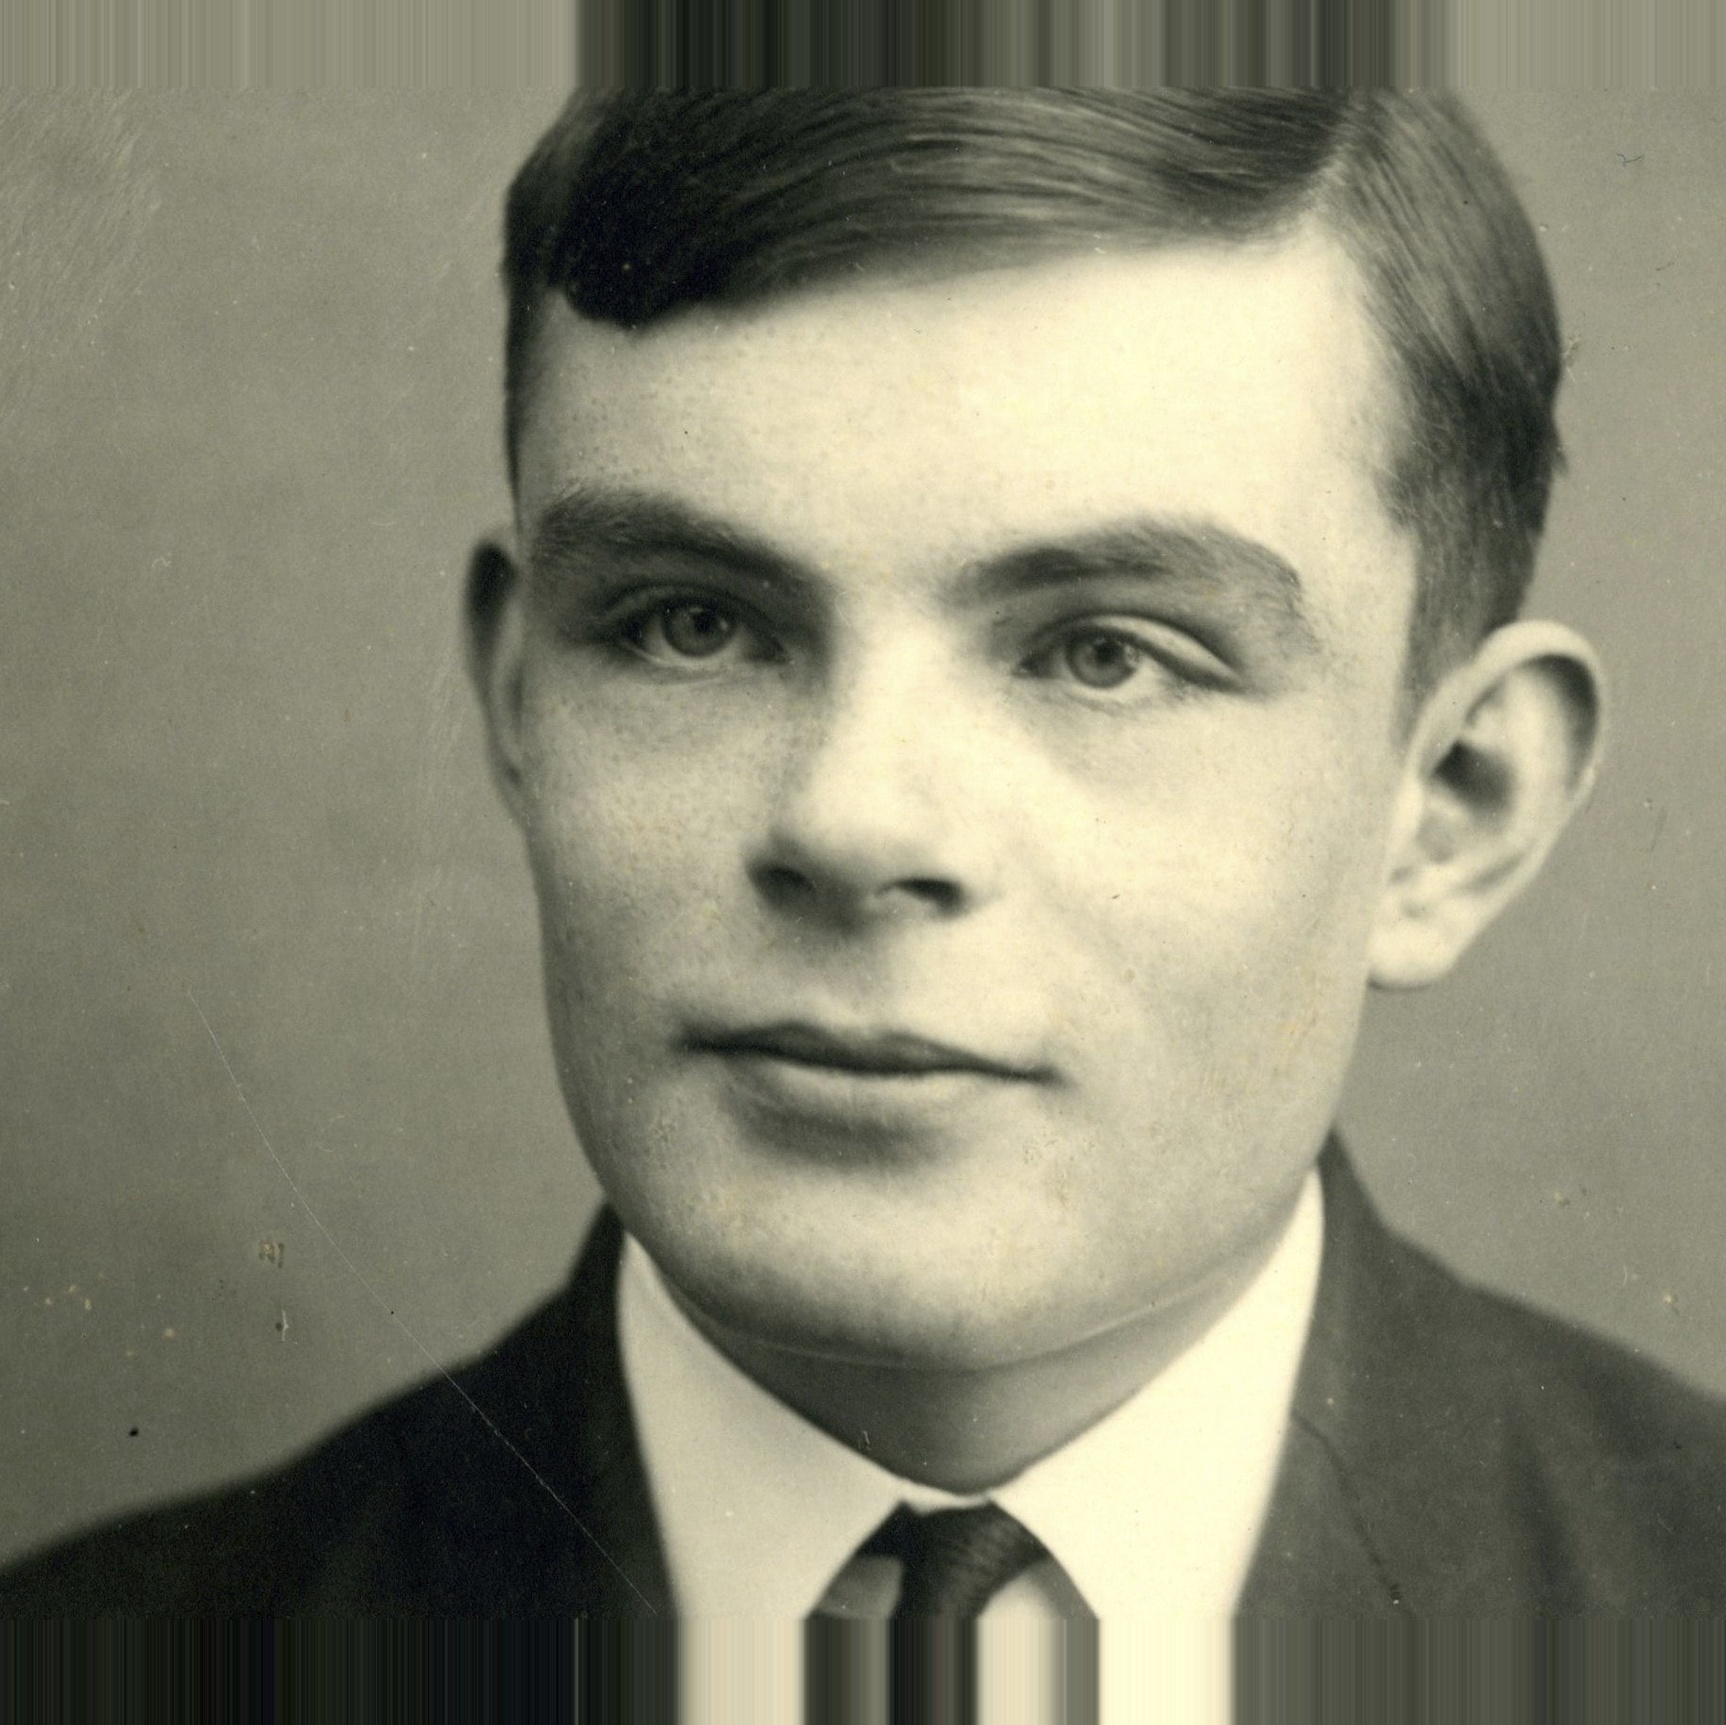
\includegraphics[height=5cm, width=\linewidth, keepaspectratio]{original_image_fgsm_1.jpg}
  \caption{Original sample classified as 28 years old}
\end{subfigure}
\begin{subfigure}{.5\textwidth}
  \centering
  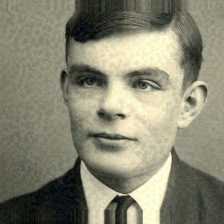
\includegraphics[height=5cm, width=\linewidth, keepaspectratio]{adversarial_image_fgsm_1.jpg}
  \caption{Adversarial sample classified as 85 years old}
\end{subfigure}

\begin{subfigure}{.5\textwidth}
  \centering
  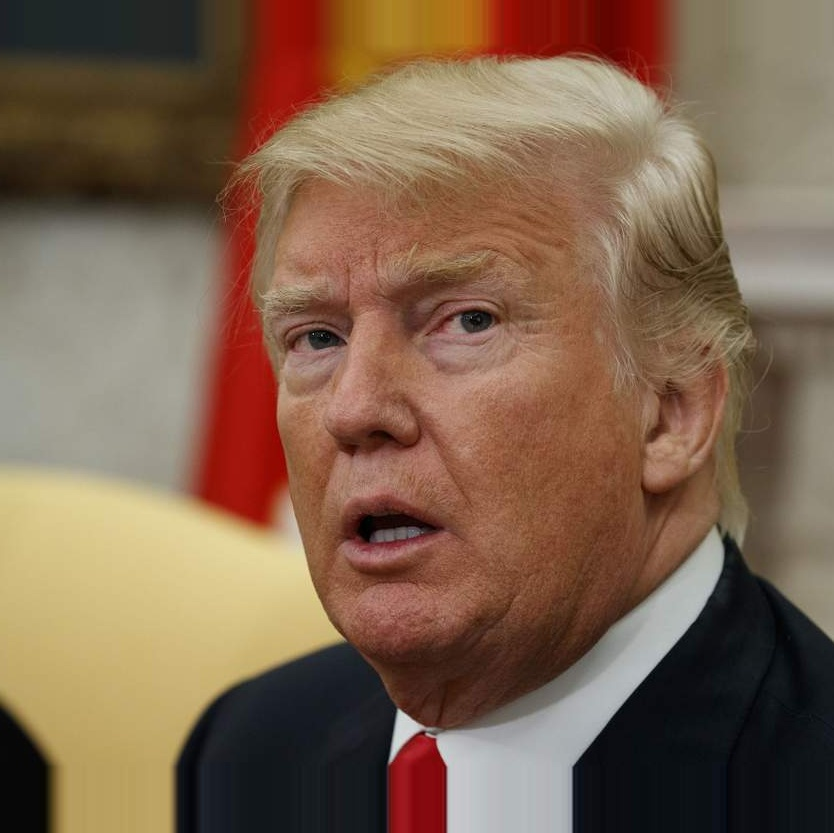
\includegraphics[height=5cm, width=\linewidth, keepaspectratio]{original_image_fgsm_2.jpg}
  \caption{Original sample classified as 59 years old}
\end{subfigure}
\begin{subfigure}{.5\textwidth}
  \centering
  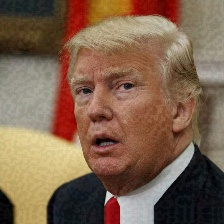
\includegraphics[height=5cm, width=\linewidth, keepaspectratio]{adversarial_image_fgsm_2.jpg}
  \caption{Adversarial sample classified as 23 years old}
\end{subfigure}

\begin{subfigure}{.5\textwidth}
  \centering
  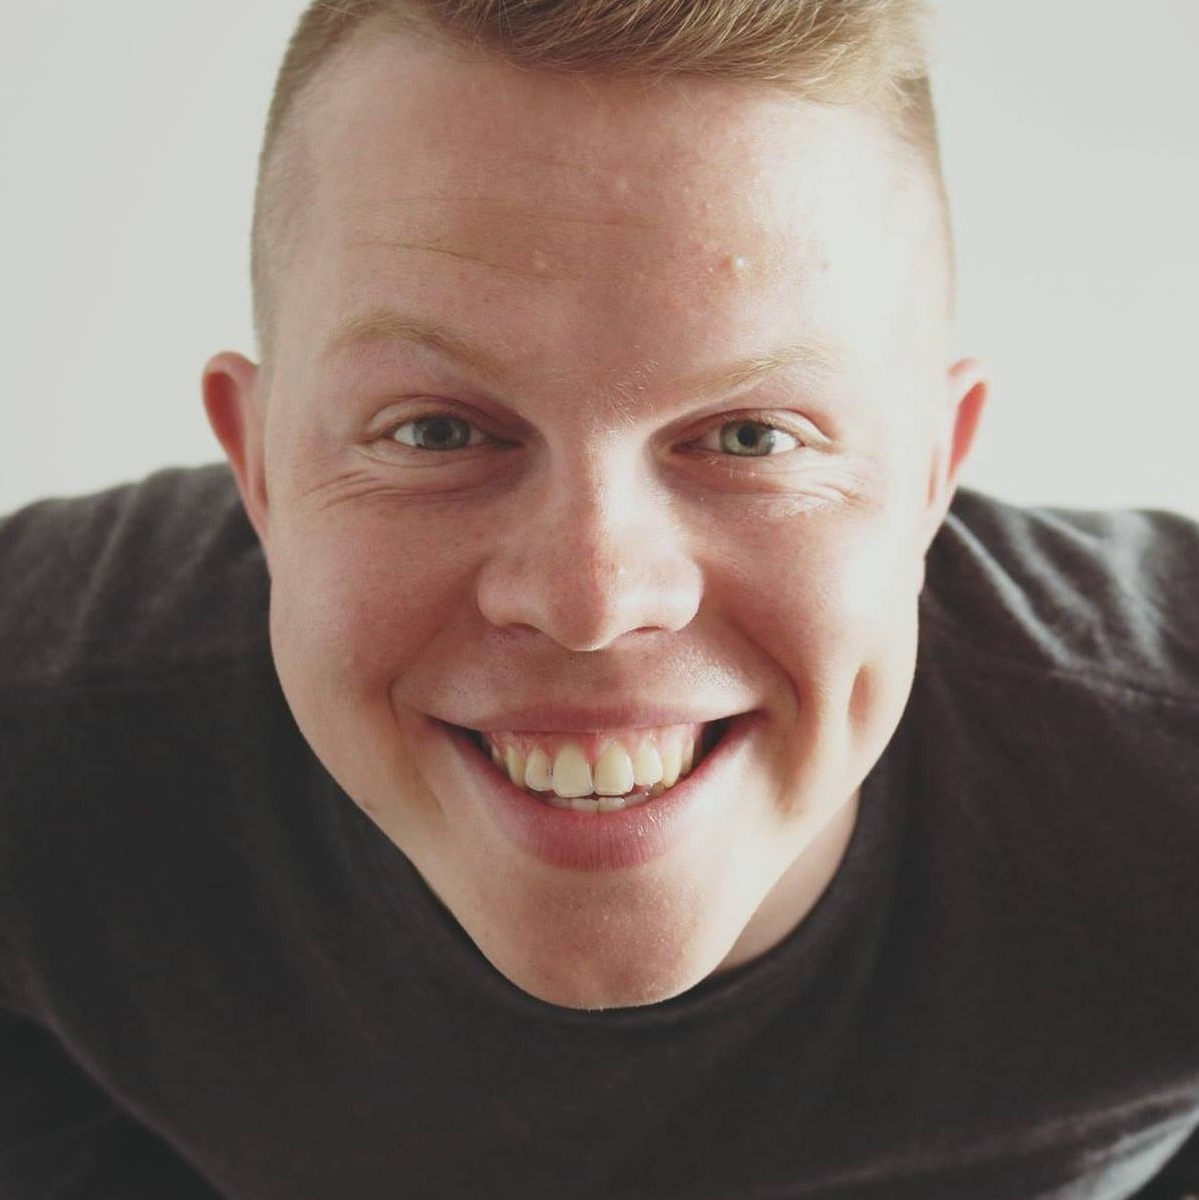
\includegraphics[height=5cm, width=\linewidth, keepaspectratio]{original_image_fgsm_3.jpg}
  \caption{Original sample classified as 28 years old}
\end{subfigure}
\begin{subfigure}{.5\textwidth}
  \centering
  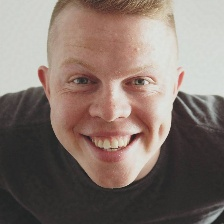
\includegraphics[height=5cm, width=\linewidth, keepaspectratio]{adversarial_image_fgsm_3.jpg}
  \caption{Adversarial sample classified as 85 years old}
\end{subfigure}

\caption{Original samples (left) and adversarial samples (right) crafted using the FGSM algorithm (\textit{eps} set to 5.0) and evaluated against the model with id 2}
\label{fig:fgsm-attack}
\end{figure}

\begin{figure}

\begin{subfigure}{.5\textwidth}
  \centering
  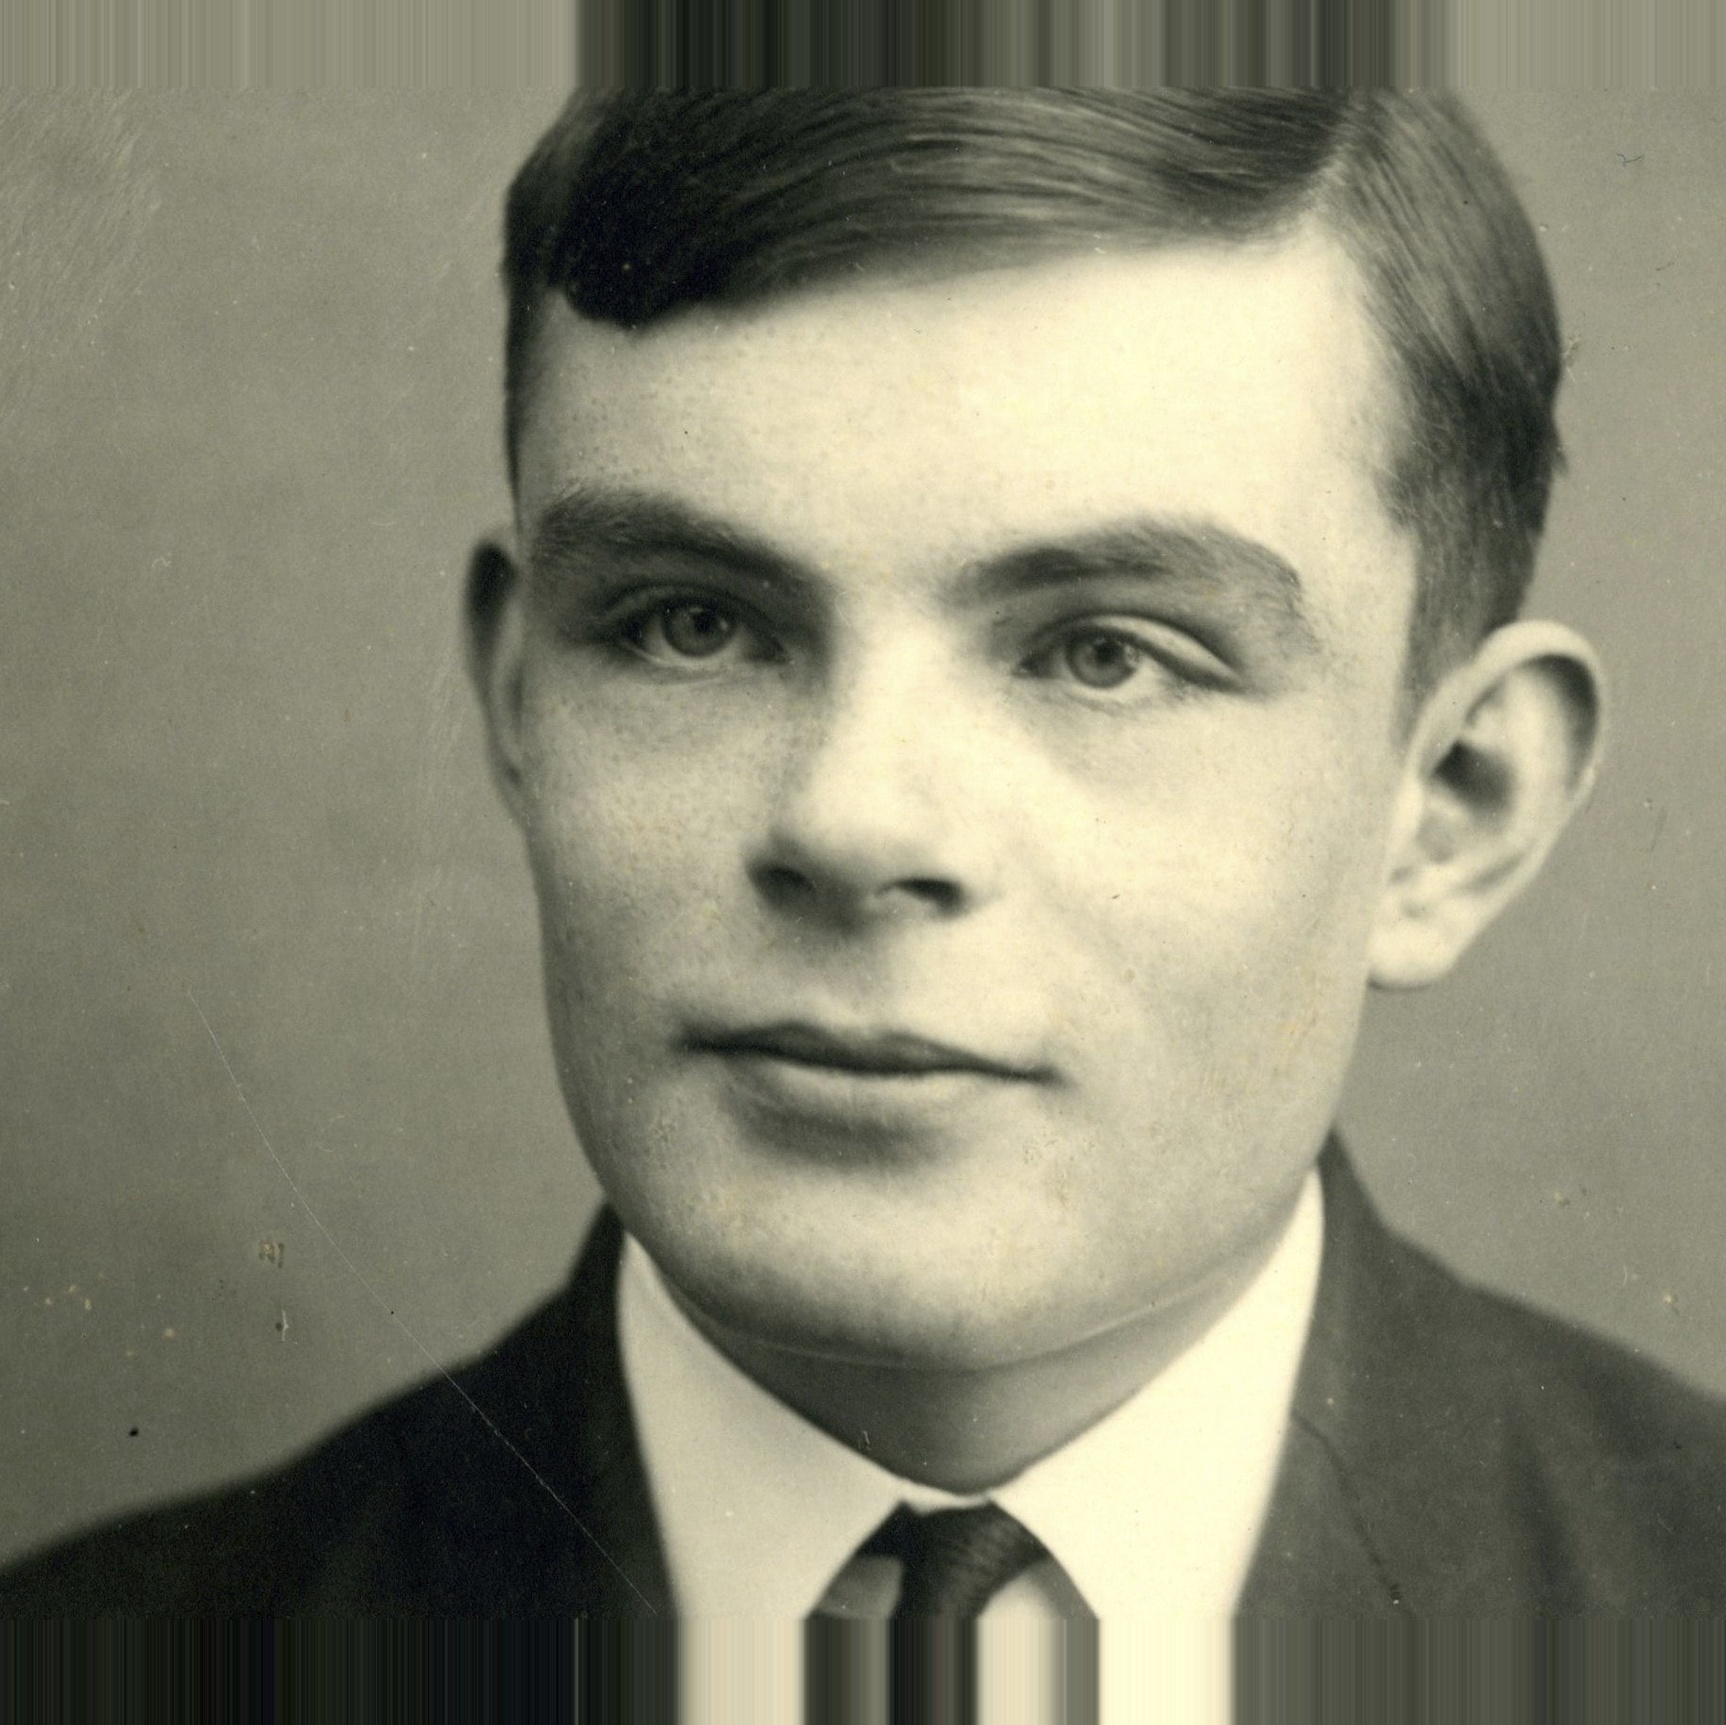
\includegraphics[height=5cm, width=\linewidth, keepaspectratio]{original_image_fgsm_1-eps1.jpg}
  \caption{Original sample classified as 28 years old}
\end{subfigure}
\begin{subfigure}{.5\textwidth}
  \centering
  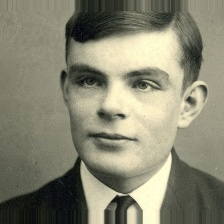
\includegraphics[height=5cm, width=\linewidth, keepaspectratio]{adversarial_image_fgsm_1-eps1.jpg}
  \caption{Adversarial sample classified as 59 years old}
\end{subfigure}

\begin{subfigure}{.5\textwidth}
  \centering
  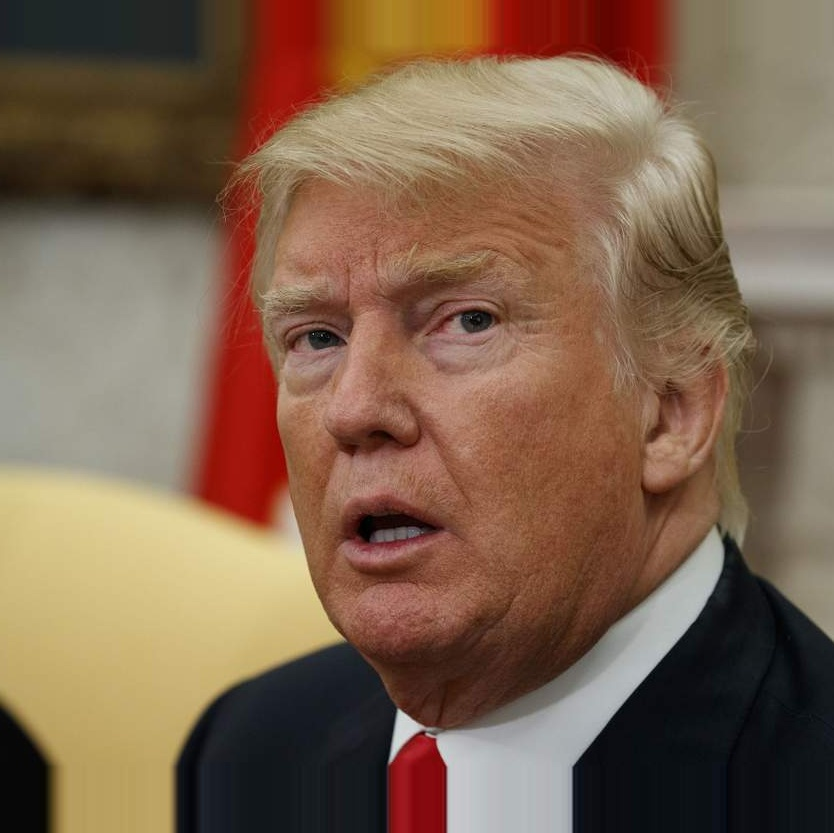
\includegraphics[height=5cm, width=\linewidth, keepaspectratio]{original_image_fgsm_2-eps1.jpg}
  \caption{Original sample classified as 59 years old}
\end{subfigure}
\begin{subfigure}{.5\textwidth}
  \centering
  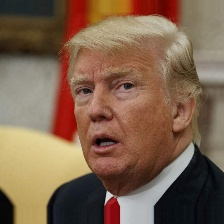
\includegraphics[height=5cm, width=\linewidth, keepaspectratio]{adversarial_image_fgsm_2-eps1.jpg}
  \caption{Adversarial sample classified as 28 years old}
\end{subfigure}

\begin{subfigure}{.5\textwidth}
  \centering
  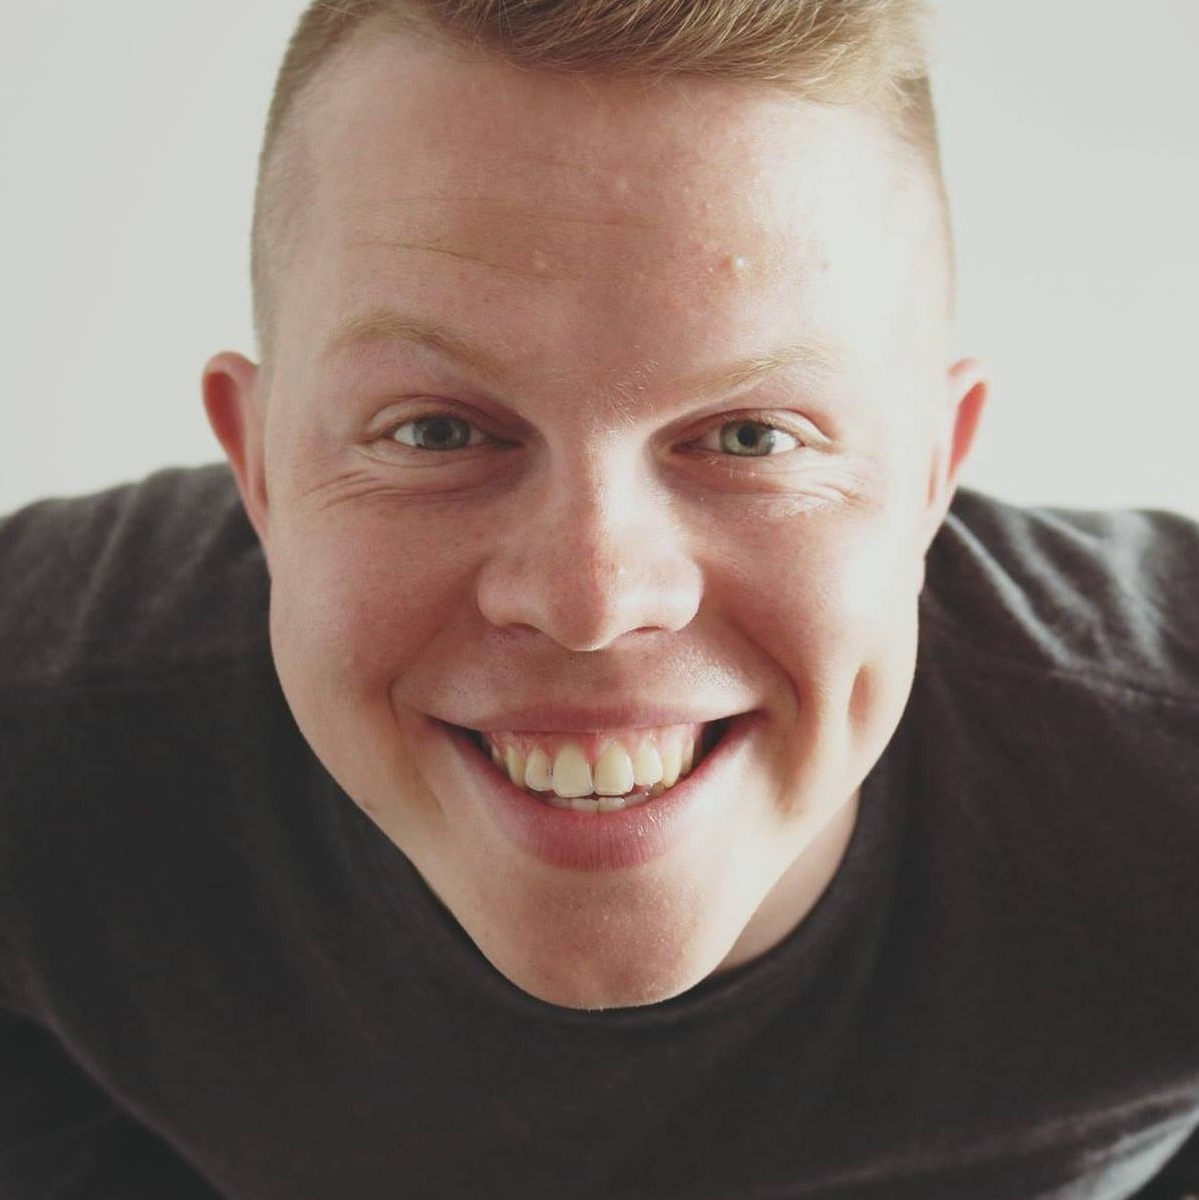
\includegraphics[height=5cm, width=\linewidth, keepaspectratio]{original_image_fgsm_3-eps1.jpg}
  \caption{Original sample classified as 28 years old}
\end{subfigure}
\begin{subfigure}{.5\textwidth}
  \centering
  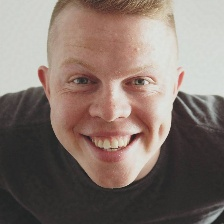
\includegraphics[height=5cm, width=\linewidth, keepaspectratio]{adversarial_image_fgsm_3-eps1.jpg}
  \caption{Adversarial sample classified as 64 years old}
\end{subfigure}

\caption{Original samples (left) and adversarial samples (right) crafted using the FGSM algorithm (\textit{eps} set to 1.0) and evaluated against the model with id 2}
\label{fig:fgsm-attack-eps1}
\end{figure}

The CW attack, given the hyperparameters in Table \ref{table:cw-params}, managed to move MAE for model with id 1 from 6.69 to 29.35. In other words, the targeted model on average predicted that a person in the adversarial image is 23 years younger or older than a person in the original image. This is not that much as FGSM managed for the model with id 2, but it is significant.

 It is also interesting to observe that amount of perturbation added to an original sample varies a lot. From value $0.00$ for minimal perturbation it can be observed that attack sometimes does not manage to find an adversarial sample and sometimes the added perturbation is rather huge. For example, maximal perturbation introduced using CW attack for model 1 is $16419.60$, but when FGSM is used, that value is $1939.89$.

Several original samples and the corresponding adversarial samples crafted in this experiment are presented in Figure \label{fig:cw-attack}. It can be observed that the attack adds a very strong pattern to every image, i.e. introduces high perturbation. This is a consequence of chosen values for number of iterations and the learning rate. 

\begin{figure}

\begin{subfigure}{.5\textwidth}
  \centering
  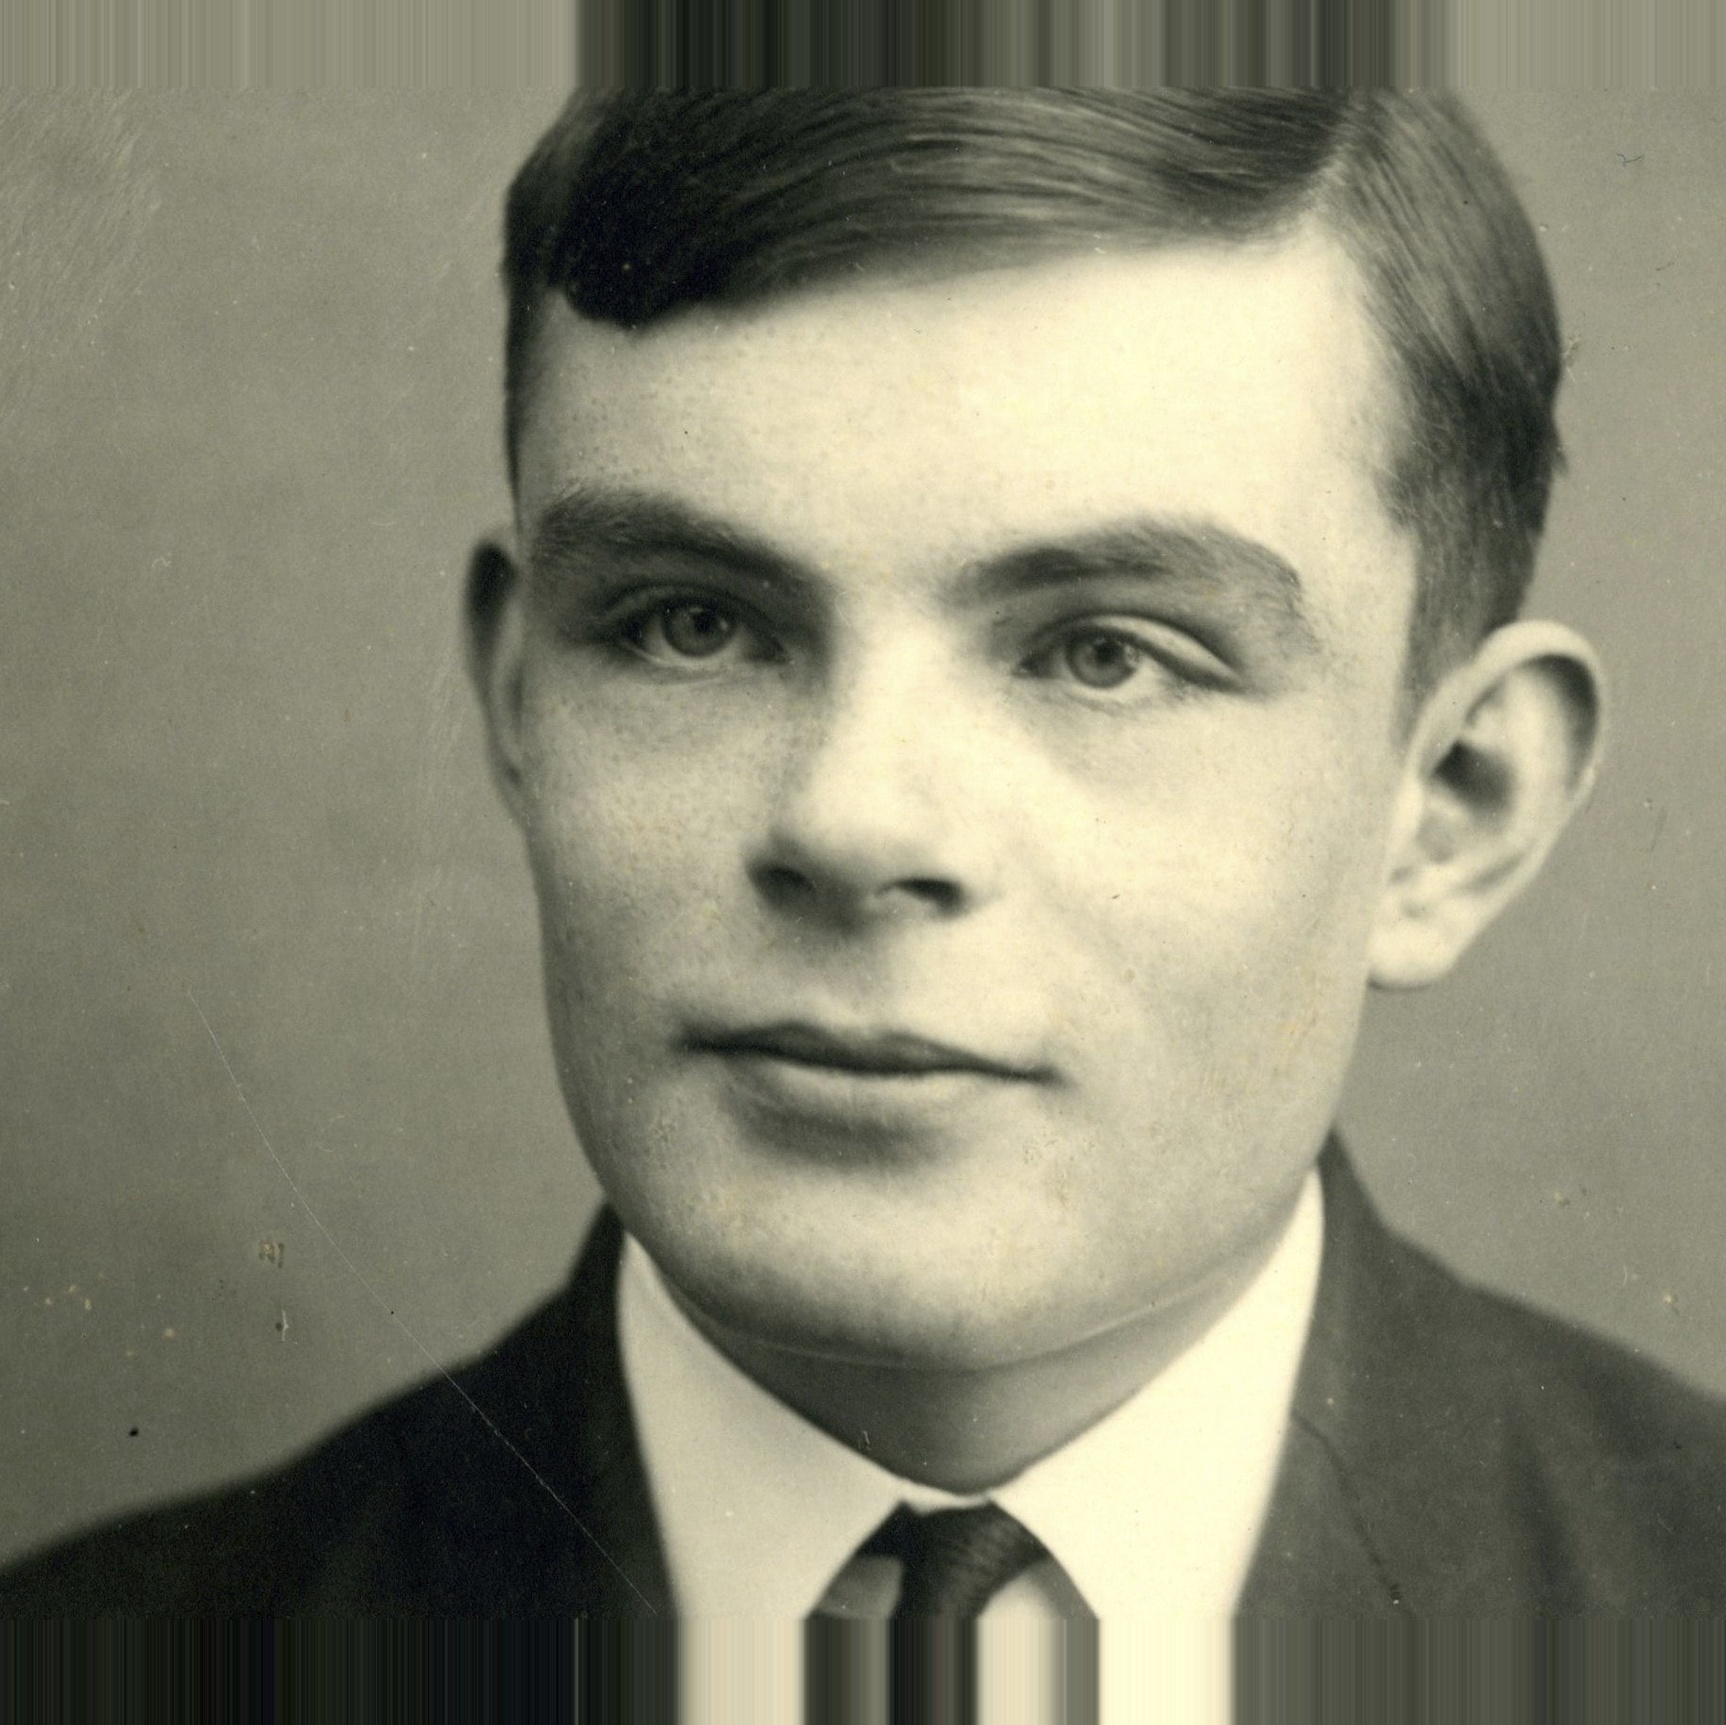
\includegraphics[height=5cm, width=\linewidth, keepaspectratio]{original_image_fgsm_1.jpg}
  \caption{Original sample classified as 36 years old}
\end{subfigure}
\begin{subfigure}{.5\textwidth}
  \centering
  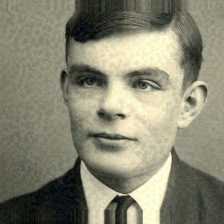
\includegraphics[height=5cm, width=\linewidth, keepaspectratio]{adversarial_image_fgsm_1.jpg}
  \caption{Adversarial sample classified as 79 years old}
\end{subfigure}

\begin{subfigure}{.5\textwidth}
  \centering
  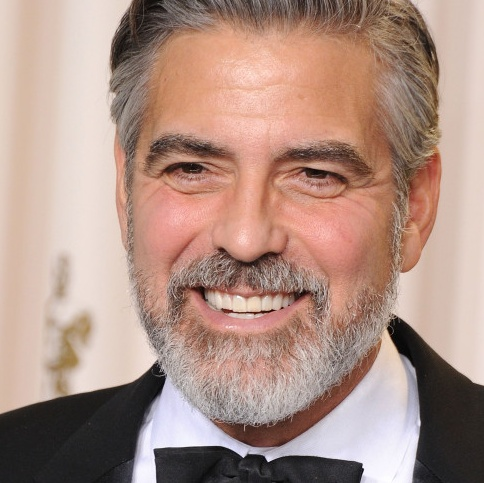
\includegraphics[height=5cm, width=\linewidth, keepaspectratio]{original_image_cw_2.jpg}
  \caption{Original sample classified as 55 years old}
\end{subfigure}
\begin{subfigure}{.5\textwidth}
  \centering
  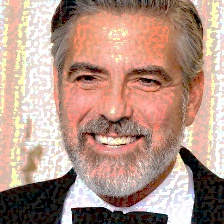
\includegraphics[height=5cm, width=\linewidth, keepaspectratio]{adversarial_image_cw_2.jpg}
  \caption{Adversarial sample classified as 10 years old}
\end{subfigure}

\begin{subfigure}{.5\textwidth}
  \centering
  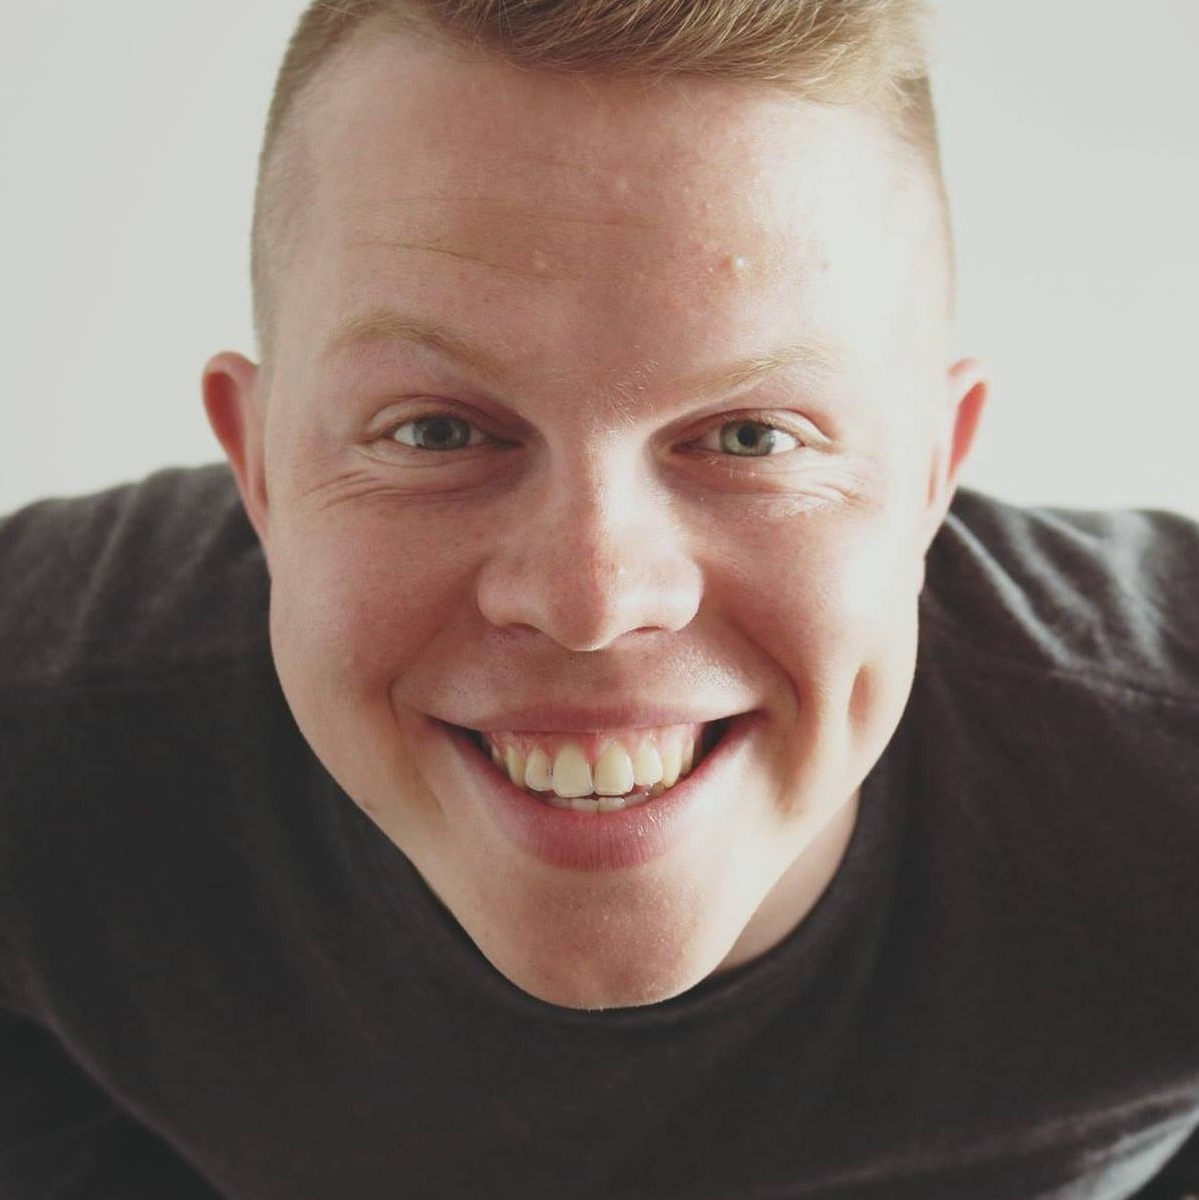
\includegraphics[height=5cm, width=\linewidth, keepaspectratio]{original_image_fgsm_3.jpg}
  \caption{Original sample classified as 35 years old}
\end{subfigure}
\begin{subfigure}{.5\textwidth}
  \centering
  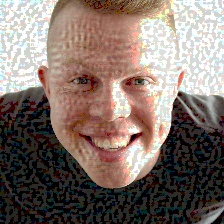
\includegraphics[height=5cm, width=\linewidth, keepaspectratio]{adversarial_image_cw_3.jpg}
  \caption{Adversarial sample classified as 84 years old}
\end{subfigure}

\caption{Original samples (left) and adversarial samples (right) crafted using the CW algorithm and evaluated against the model with id 1}
\label{fig:cw-attack}
\end{figure}


Since CW attack wasn't able to find any adversarial sample for the model with id 2 with the given hyperparameters in Table \ref{table:cw-params}, further experiments are performed against that model with different values for learning rate and maximum number of iterations.

Results of those experiments are presented in Table \ref{table:cw-results}. The results show that it is not easy for CW attack to find any adversarial sample on a specific model. Although no adversarial sample is found, I performed no further exploration of combination of learning rate and number of iterations. Further argumentation of this decision can be found in Section \ref{sec:threats-to-validity}.

It is also interesting to notice that for models with id 1 and 2, the attacks find stronger adversarial samples (i.e. bigger change in MAE) than for models with id 3 and 4. Could it be that bigger models \footnote{ResNet50 architecture that is used for model 1 and 2 has 25,636,712 parameters and InceptionResNetV2  architecture that is used for model 3 and 4 has 55,873,736 parameters.} are more resistent to adversarial samples? 

As expected from the analysis of the paper \cite{DBLP:journals/corr/CarliniW16a} in Section \ref{sec:CW}, JSMA attack failed due to memory complexity of the algorithm.

\begin{table}[]
\centering
\begin{tabular}{|c|c|}
\hline
eps & 5 \\  \hline
clip min & 0  \\ \hline
clip max & 255 \\ \hline
y\_target & 10 or 90 \\ \hline
\end{tabular}
\caption{Values of the hyperparameters used in the FGSM attack}
\label{table:fgsm-params}
\end{table}

\begin{table}[]
\centering
\begin{tabular}{|c|c|}
\hline
binary\_search\_steps & 8 \\ \hline
y\_target & 10 or 90 \\ \hline
abort\_early & True \\ \hline
max\_iterations & 5000 \\ \hline
learning\_rate & 1 \\ \hline
clip\_max & 255 \\ \hline
clip\_min & 0 \\ \hline
initial\_const & 0.1 \\ \hline
\end{tabular}
\caption{Values of the hyperparameters  used in the CW attack}
\label{table:cw-params}
\end{table}

\begin{table}[]
\centering
\begin{tabular}{|cccccccc|}
\hline
\multicolumn{2}{|c|}{} & \multicolumn{2}{c|}{FGSM} & \multicolumn{2}{c|}{CW} & \multicolumn{2}{c|}{JSMA} \\ \hline
\multicolumn{1}{|c|}{\begin{tabular}[c]{@{}c@{}}model\\ id\end{tabular}} & \multicolumn{1}{c|}{\begin{tabular}[c]{@{}c@{}}clean\\ MAE\end{tabular}} & \multicolumn{1}{c|}{\begin{tabular}[c]{@{}c@{}}adv\\ MAE\end{tabular}} & \multicolumn{1}{c|}{\begin{tabular}[c]{@{}c@{}}avg\\ L2\end{tabular}} & \multicolumn{1}{c|}{\begin{tabular}[c]{@{}c@{}}adv\\ MAE\end{tabular}} & \multicolumn{1}{c|}{\begin{tabular}[c]{@{}c@{}}avg\\ L2\end{tabular}} & \multicolumn{1}{c|}{\begin{tabular}[c]{@{}c@{}}adv\\ MAE\end{tabular}} & \multicolumn{1}{c|}{\begin{tabular}[c]{@{}c@{}}avg\\ L2\end{tabular}} \\ \hline
1 & 6.69 & 32.25 & 1879.63 & 29.35 & 2977.28 & - & - \\ \hline
2 & 9.50 & 47.79 & 1879.49 & 9.50 & 0.00 & - & - \\ \hline
3 & 5.40 & 19.32 & 2510.92 & 7.51 & 1307.51 & - & - \\ \hline
4 & 4.62 & 15.03 & 2511.10 & 6.79 & 1104.78 & - & - \\ \hline
\end{tabular}
\caption{Results of different adversarial attacks. The "-" sign means that an attack couldn't be executed.}
\label{table:whitebox-results}
\end{table}

% Please add the following required packages to your document preamble:
% \usepackage{graphicx}
\begin{table}[]
\resizebox{\textwidth}{!}{%
\begin{tabular}{|c|c|c|c|c|c|c|}
\hline
model id & clean MAE & adv MAE & avg L2 & std dev L2 & min L2 & max L2 \\ \hline
1 & 6.69 & 32.25 & 1879.63 & 77.23  & 1637.33 & 1939.89  \\ \hline
2 & 9.50 & 47.79 & 1879.49 & 77.26 & 1649.43 & 1939.90 \\ \hline
3 & 5.40 & 19.32 & 2510.92 &  100.00 & 2201.44 & 2589.42  \\ \hline
4 & 4.62 & 15.08 & 2511.10 & 99.53 & 2204.20 & 2589.41 \\ \hline
\end{tabular}%
}
\caption{Results of FGSM attack}
\label{table:whitebox-fgsm-results}
\end{table}

% Please add the following required packages to your document preamble:
% \usepackage{graphicx}
\begin{table}[]
\resizebox{\textwidth}{!}{%
\begin{tabular}{|c|c|c|c|c|c|c|}
\hline
model id & clean MAE & adv MAE & avg L2 & std dev L2 & min L2 & max L2 \\ \hline
1 & 6.69 & 29.35 & 2977.28 & 3532.85 & 0.0 & 16419.60 \\ \hline
2 & 9.50 & 9.50 & 0.00 & 0.00 & 0.00 &  \\ \hline
3 & 5.40 & 7.51 & 1307.51 & 2969.74 & 0.00 & 11071.88  \\ \hline
4 & 4.62 & 6.79 & 1104.78 & 3070.10 & 0.00 & 17673.81  \\ \hline
\end{tabular}%
}
\caption{Results of CW attack}
\label{table:whitebox-cw-results}
\end{table}

\begin{table}[]
\begin{tabular}{|c|c|c|c|c|}
\hline
max iterations & learning rate & clean MAE & adv MAE & avg L2 \\ \hline
5 000 & 1 & 9.5 & 9.5 & 0.0 \\ \hline
10 000 & 1 & 9.5 & 9.5 & 0.0  \\ \hline
10 000 & 0.1 & 9.5 & 9.5 & 0.0 \\ \hline
10 000 & 10.0 & 9.5 & 9.5 & 0.0 \\ \hline
100 000 & 0.01 & 9.5 & 9.5 & 0.0 \\ \hline
\end{tabular}
\caption{Results using the CW attack with different values of hyperparameters against model with id 2}
\label{table:cw-results}
\end{table}